% SW403 Course Project -- Phase 2: Experimentation & Prototype Development
% Compile on Overleaf (pdfLaTeX). Results numbers come from results/summary.md.
\documentclass[conference]{IEEEtran}
\usepackage{cite}
\usepackage{amsmath}
\usepackage{booktabs}
\usepackage{graphicx}
\usepackage{url}

\begin{document}

\title{Phase 2: Prototype, Experimental Setup and Early Results\\
Does Multi-Agent Collaboration Really Help LLM Bug Fixing?}

\author{
\IEEEauthorblockN{Seif Zaki}
\IEEEauthorblockA{Zewail City of Science and Technology\\ ID: 202201554}
\and
\IEEEauthorblockN{Karim Wael}
\IEEEauthorblockA{Zewail City of Science and Technology\\ ID: 202202212}
\and
\IEEEauthorblockN{Ahmed Ayman}
\IEEEauthorblockA{Zewail City of Science and Technology\\ ID: 202200168}
}

\maketitle

\begin{abstract}
We implemented the prototype proposed in Phase 1: four LLM repair systems that
share a hard per-bug budget of LLM calls and output tokens --- a single-shot
baseline (S0), a single agent with test feedback (S1), a LangGraph multi-agent
pipeline with localiser, fixer, test-runner tool and reviewer (S2), and S2
without the reviewer (S2$-$R). An automatic evaluator runs every final patch in
a sandbox against \emph{held-out} tests the systems never see, separating
correct from plausible-but-incorrect patches and flagging five hallucination
types. We report early results on 31 QuixBugs Python bugs with Gemini 3.5
Flash-Lite, three runs per bug and system. In the 228 attempts completed so far, all four systems fix 96--98\% of bugs, the multi-agent pipeline costs 3.3$\times$ the output tokens of the single agent for one extra fix, and the only failures are plausible-but-incorrect patches that pass every visible test.
\end{abstract}

\section{Changes Since Phase 1}
\begin{itemize}
\item \textbf{Model.} We use \texttt{gemini-3.5-flash-lite} through Google's
OpenAI-compatible endpoint (free tier, 15 requests/minute). The code is
provider-neutral: any OpenAI-compatible endpoint is one setting.
\item \textbf{Dataset scope.} Phase 2 uses the 31 QuixBugs Python programs that
ship JSON test cases. The 9 graph programs (which use \texttt{node.py}
objects) are excluded and listed in the dataset manifest. ConDefects and the
identifier-renaming probe (RQ3) move to Phase 3.
\item \textbf{Budget.} Each bug gets at most $K=8$ LLM calls and $T=8000$
output tokens. Rate-limit retries are not charged; only completed calls count.
\end{itemize}

\section{Prototype Implementation}
The replication package is the GitHub repository (Section~\ref{sec:repl}).
\begin{itemize}
\item \textbf{Budgeted model client} (\texttt{bugfix/llm.py}). Every system
calls the model only through one client that charges a shared \texttt{Budget}
and raises \texttt{BudgetExceeded} when calls or output tokens run out, so the
equal-budget condition of RQ1 is enforced, not assumed.
\item \textbf{Repair systems} (\texttt{bugfix/systems/}). All systems receive
the same information: the buggy function, the visible tests and the buggy
program's results on them. S0 makes one call. S1 is one growing conversation:
patch, run visible tests, return the failures, repeat. S2 is a LangGraph state
graph: Localiser $\rightarrow$ Fixer $\rightarrow$ Test-runner (a deterministic
tool, not an LLM) $\rightarrow$ Reviewer; failed tests or a rejection loop back
to the Fixer. S2$-$R stops as soon as the visible tests pass.
\item \textbf{Sandbox} (\texttt{bugfix/sandbox.py}, \texttt{harness.py}).
Candidate code runs in a separate isolated Python process (\texttt{python -I})
with a per-test timeout, a 1~GiB memory limit and its own temporary directory.
\item \textbf{Evaluation module} (\texttt{bugfix/evaluate.py}). Labels each
final patch \emph{correct} (passes visible and held-out tests),
\emph{plausible-but-incorrect} (passes visible tests only) or \emph{failing},
and flags hallucinations: H1 non-runnable code, H2 non-existent API or
third-party import, H3 changed function signature, H4 unchanged code returned,
H5 reviewer approval of a patch that fails held-out tests.
\item \textbf{Service and dashboard.} A FastAPI endpoint \texttt{POST /repair}
runs any system on submitted code and tests and returns the patch, label,
usage and agent trace. A Streamlit dashboard shows outcome rates,
hallucination flags, McNemar tests, reviewer accuracy, errors and the full
trace of any attempt.
\item \textbf{Tests.} 44 automated tests: plumbing tests with a scripted model
(no API calls), and a dataset check that every reference fix is labelled
correct and every buggy program failing.
\end{itemize}

\section{Experimental Setup and Dataset}
\textbf{Data.} QuixBugs~\cite{quixbugs} (MIT licence, commit \texttt{4257f44}).
For each program we keep the tests the reference program passes (two slow
tests, also skipped by the official suite, are dropped), discard bugs the
buggy program does not fail, and split the tests with a fixed seed: about half
of the failing and half of the passing tests become visible, the rest are
held out. All 31 bugs have at least one visible failing test and at least one
held-out test (240 tests: 118 visible, 122 held-out). \texttt{sqrt} is compared with the
tolerance used by the official tests.

\textbf{Design.} 31 bugs $\times$ 4 systems $\times$ 3 runs = 372 attempts,
temperature 0.2, same model and budget for all systems.

\textbf{Metrics and statistics.} Correct-fix rate with 95\% bootstrap
confidence intervals over bugs; plausible-but-incorrect rate and overfitting
rate (plausible-but-incorrect / all visible-passing); hallucination rates;
calls and tokens per attempt. Systems are compared with exact McNemar tests on
paired (bug, run) correctness.

\section{Early Results}
\textbf{Status.} The free tier allows 500 requests per day, so the run is
split over two days. These results cover 228 of 372 attempts (runs 1--2 of 3);
the final numbers will replace them in the repository and in Phase 3.

\begin{table}[h]
\caption{Early results, 31 QuixBugs bugs, gemini-3.5-flash-lite}
\label{tab:res}
\centering
\footnotesize
\begin{tabular}{@{}lccccc@{}}
\toprule
System & Att. & Correct [95\% CI] & Pl.-incorr. & Calls & Out tok \\
\midrule
S0 single-shot & 57 & 0.965 [0.90, 1.00] & 0.035 & 1.00 & 110 \\
S1 single agent & 58 & 0.966 [0.90, 1.00] & 0.034 & 1.00 & 106 \\
S2 multi-agent & 56 & 0.982 [0.95, 1.00] & 0.018 & 3.79 & 355 \\
S2$-$R no reviewer & 57 & 0.965 [0.90, 1.00] & 0.035 & 2.11 & 189 \\
\bottomrule
\end{tabular}
\end{table}

\begin{figure}[h]
\centering
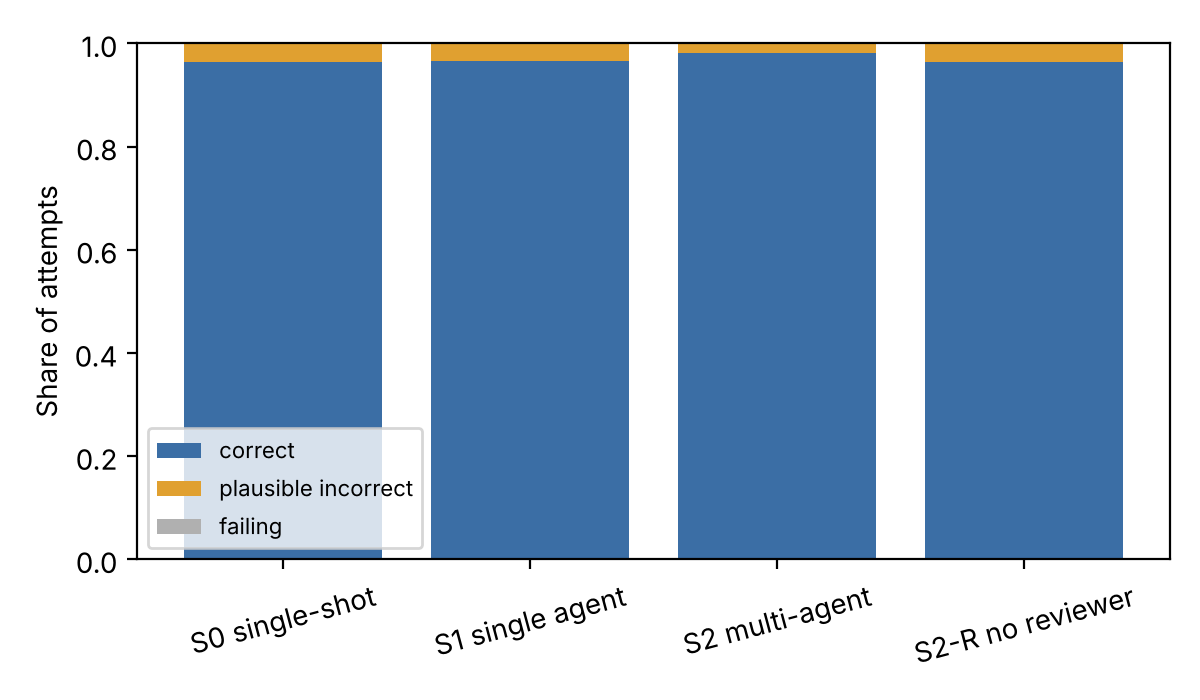
\includegraphics[width=\columnwidth]{../../results/figures/outcomes.png}
\caption{Outcome of each attempt: correct, plausible-but-incorrect, failing.}
\end{figure}

\textbf{RQ1 (equal budget).} All systems are at the ceiling (Table~\ref{tab:res}).
S2 is correct on one more (bug, run) pair than S1; exact McNemar $p=1.0$, so there
is no evidence of a difference. S2 spends 3.8 calls and 3.3$\times$ the output
tokens of S1 per attempt. S1 never needed a second call: every first patch passed
the visible tests, so on QuixBugs the test-feedback loop is never exercised and
S0 and S1 are equivalent. QuixBugs therefore cannot separate the systems, as
anticipated in Phase 1; ConDefects is needed.

\textbf{RQ2 (reviewer).} The reviewer issued 20 rejections over 56 S2 attempts,
mostly of patches later approved in another form; 6 attempts used the whole
budget of 8 calls. Of the 52 final patches it judged, it approved 50 correct ones,
approved 1 wrong one (H5) and rejected 1 correct one; it caught none of the wrong
patches. Removing it (S2$-$R) lost one fix and halved the cost.

\textbf{Hallucination and overfitting.} No patch was non-runnable, used a
non-existent API, changed the signature or returned the code unchanged (H1--H4 =
0). All failures are on \texttt{max\_sublist\_sum}: every system replaced the
buggy line with the textbook Kadane variant that returns the largest element
for an all-negative list ($-4$ for \texttt{[-4,-4,-5]}), while the function's
docstring allows the empty sublist (answer 0). The patch passes all three
visible tests and fails a held-out one: a plausible-but-incorrect patch produced
from a memorised algorithm rather than the specification, and the S2 reviewer
approved it once. This is the failure mode the held-out tests were designed to
catch~\cite{quixbugs}.


\section{Threats to Validity}
QuixBugs is public, saturated~\cite{gpto1} and likely in the model's training
data, so absolute fix rates overstate repair ability; RQ3 (renaming) and
ConDefects in Phase 3 address this. Held-out tests are a proxy for correctness:
a patch can pass them and still be wrong, so Phase 3 adds a manual check of a
sample against the reference fix. With 31 bugs, differences of a few bugs are
not statistically meaningful. Budget matching counts calls and output tokens,
not prompt tokens, which differ between systems.

\section{Plan for Phase 3}
(1) ConDefects-Python sample and the identifier-renaming probe (RQ3);
(2) manual correctness check of 20\% of plausible patches by two members with
Cohen's $\kappa$; (3) mapping S2 failures to MAST categories~\cite{mast};
(4) a second model to test generality, if quota allows; (5) the final paper.

\section{Replication Package}\label{sec:repl}
\url{https://github.com/seif-356/AI_modern_software} (branch \texttt{phase-2}):
code (\texttt{bugfix/}), dataset (\texttt{data/quixbugs/}), results generation
scripts (\texttt{scripts/}), raw and aggregated results (\texttt{results/}),
dashboard and tests. The README lists the commands to reproduce every number.

\section*{AI Tools Declaration}
% TODO: update to reflect what the team actually used.
Claude Code (Anthropic) was used to implement the prototype and draft this
report. Gemini 3.5 Flash-Lite is the model under study. All content was
reviewed by the authors.

\begin{thebibliography}{9}
\bibitem{quixbugs}
D.~Lin, J.~Koppel, A.~Chen, and A.~Solar-Lezama, ``QuixBugs: A multi-lingual
program repair benchmark set based on the Quixey challenge,'' in \emph{Proc.
SPLASH Companion}, 2017.
\bibitem{gpto1}
H.~Hu, Y.~Shang, G.~Xu, C.~He, and Q.~Zhang, ``Can GPT-O1 kill all bugs? An
evaluation of GPT-family LLMs on QuixBugs,'' in \emph{Proc. APR Workshop}, 2025.
\bibitem{mast}
M.~Cemri, M.~Pan \emph{et al.}, ``Why do multi-agent LLM systems fail?'' in
\emph{Proc. NeurIPS}, 2025.
\end{thebibliography}

\end{document}
